\documentclass[12pt]{article} 
% \documentclass[12pt]{amsart} 

% Custom definitions
% To use this customization file, insert the line "% Custom definitions
% To use this customization file, insert the line "% Custom definitions
% To use this customization file, insert the line "\input{custom}" in the header of the tex file.

% Formatting

\tolerance=1000
\usepackage[margin=1in]{geometry}


% Packages

% \usepackage{amssymb,latexsym}
\usepackage{amssymb,amsfonts,amsmath,latexsym,amsthm}
\usepackage[usenames,dvipsnames]{color}
\usepackage[]{graphicx}
\usepackage[space]{grffile}
\usepackage{mathrsfs}   % fancy math font
% \usepackage[font=small,skip=0pt]{caption}
\usepackage[skip=0pt]{caption}
\usepackage{subcaption}
\usepackage{verbatim}
\usepackage{url}
\usepackage{bm}
\usepackage{dsfont}
\usepackage{extarrows}
\usepackage{multirow}
% \usepackage{wrapfig}
% \usepackage{epstopdf}
\usepackage{rotating}
\usepackage{tikz}
\usetikzlibrary{fit}					% fitting shapes to coordinates
%\usetikzlibrary{backgrounds}	% drawing the background after the foreground

\usepackage{fancyhdr}

\fancypagestyle{firststyle}{
   \fancyhf{}
   \renewcommand{\footrulewidth}{0.4pt}
   \fancyfoot[L]{\footnotesize This work is licensed under a \href{http://creativecommons.org/licenses/by-nc-nd/4.0/}{Creative Commons BY-NC-ND 4.0 International License}.\\ Jeffrey W. Miller (2015). \textit{Lecture Notes on Bayesian Statistics}. Duke University, Durham, NC.}
}


% \usepackage[dvipdfm,colorlinks,citecolor=blue,linkcolor=blue,urlcolor=blue]{hyperref}
\usepackage[colorlinks,citecolor=blue,linkcolor=blue,urlcolor=blue]{hyperref}
%\usepackage{hyperref}
\usepackage[authoryear,round]{natbib}


%  Theorems, etc.

\theoremstyle{plain}
\newtheorem{theorem}{Theorem}[section]
\newtheorem{corollary}[theorem]{Corollary}
\newtheorem{lemma}[theorem]{Lemma}
\newtheorem{proposition}[theorem]{Proposition}
\newtheorem{condition}[theorem]{Condition}
% \newtheorem{conditions}[theorem]{Conditions}

\theoremstyle{definition}
\newtheorem{definition}[theorem]{Definition}
% \newtheorem*{unnumbered-definition}{Definition}
\newtheorem{example}[theorem]{Example}
\theoremstyle{remark}
\newtheorem*{remark}{Remark}
\numberwithin{equation}{section}



% Document-specific shortcuts
\newcommand{\btheta}{{\bm\theta}}
\newcommand{\bbtheta}{{\pmb{\bm\theta}}}

\newcommand{\commentary}[1]{\ifx\showcommentary\undefined\else \emph{#1}\fi}

\newcommand{\term}[1]{\textit{\textbf{#1}}}

% Math shortcuts

% Probability distributions
\DeclareMathOperator*{\Exp}{Exp}
\DeclareMathOperator*{\TExp}{TExp}
\DeclareMathOperator*{\Bernoulli}{Bernoulli}
\DeclareMathOperator*{\Beta}{Beta}
\DeclareMathOperator*{\Ga}{Gamma}
\DeclareMathOperator*{\TGamma}{TGamma}
\DeclareMathOperator*{\Poisson}{Poisson}
\DeclareMathOperator*{\Binomial}{Binomial}
\DeclareMathOperator*{\NormalGamma}{NormalGamma}
\DeclareMathOperator*{\InvGamma}{InvGamma}
\DeclareMathOperator*{\Cauchy}{Cauchy}
\DeclareMathOperator*{\Uniform}{Uniform}
\DeclareMathOperator*{\Gumbel}{Gumbel}
\DeclareMathOperator*{\Pareto}{Pareto}
\DeclareMathOperator*{\Mono}{Mono}
\DeclareMathOperator*{\Geometric}{Geometric}
\DeclareMathOperator*{\Wishart}{Wishart}

% Math operators
\DeclareMathOperator*{\argmin}{arg\,min}
\DeclareMathOperator*{\argmax}{arg\,max}
\DeclareMathOperator*{\Cov}{Cov}
\DeclareMathOperator*{\diag}{diag}
\DeclareMathOperator*{\median}{median}
\DeclareMathOperator*{\Vol}{Vol}

% Math characters
\newcommand{\R}{\mathbb{R}}
\newcommand{\Z}{\mathbb{Z}}
\newcommand{\E}{\mathbb{E}}
\renewcommand{\Pr}{\mathbb{P}}
\newcommand{\I}{\mathds{1}}
\newcommand{\V}{\mathbb{V}}

\newcommand{\A}{\mathcal{A}}
\newcommand{\C}{\mathcal{C}}
\newcommand{\D}{\mathcal{D}}
\newcommand{\Hcal}{\mathcal{H}}
\newcommand{\M}{\mathcal{M}}
\newcommand{\N}{\mathcal{N}}
\newcommand{\X}{\mathcal{X}}
\newcommand{\Zcal}{\mathcal{Z}}
\renewcommand{\P}{\mathcal{P}}

\newcommand{\T}{\mathtt{T}}
\renewcommand{\emptyset}{\varnothing}


% Miscellaneous commands
\newcommand{\iid}{\stackrel{\mathrm{iid}}{\sim}}
\newcommand{\matrixsmall}[1]{\bigl(\begin{smallmatrix}#1\end{smallmatrix} \bigr)}

\newcommand{\items}[1]{\begin{itemize} #1 \end{itemize}}

\newcommand{\todo}[1]{\emph{\textcolor{red}{(#1)}}}

\newcommand{\branch}[4]{
\left\{
	\begin{array}{ll}
		#1  & \mbox{if } #2 \\
		#3 & \mbox{if } #4
	\end{array}
\right.
}

% approximately proportional to
\def\app#1#2{%
  \mathrel{%
    \setbox0=\hbox{$#1\sim$}%
    \setbox2=\hbox{%
      \rlap{\hbox{$#1\propto$}}%
      \lower1.3\ht0\box0%
    }%
    \raise0.25\ht2\box2%
  }%
}
\def\approxprop{\mathpalette\app\relax}

% \newcommand{\approptoinn}[2]{\mathrel{\vcenter{
  % \offinterlineskip\halign{\hfil$##$\cr
    % #1\propto\cr\noalign{\kern2pt}#1\sim\cr\noalign{\kern-2pt}}}}}

% \newcommand{\approxpropto}{\mathpalette\approptoinn\relax}





" in the header of the tex file.

% Formatting

\tolerance=1000
\usepackage[margin=1in]{geometry}


% Packages

% \usepackage{amssymb,latexsym}
\usepackage{amssymb,amsfonts,amsmath,latexsym,amsthm}
\usepackage[usenames,dvipsnames]{color}
\usepackage[]{graphicx}
\usepackage[space]{grffile}
\usepackage{mathrsfs}   % fancy math font
% \usepackage[font=small,skip=0pt]{caption}
\usepackage[skip=0pt]{caption}
\usepackage{subcaption}
\usepackage{verbatim}
\usepackage{url}
\usepackage{bm}
\usepackage{dsfont}
\usepackage{extarrows}
\usepackage{multirow}
% \usepackage{wrapfig}
% \usepackage{epstopdf}
\usepackage{rotating}
\usepackage{tikz}
\usetikzlibrary{fit}					% fitting shapes to coordinates
%\usetikzlibrary{backgrounds}	% drawing the background after the foreground

\usepackage{fancyhdr}

\fancypagestyle{firststyle}{
   \fancyhf{}
   \renewcommand{\footrulewidth}{0.4pt}
   \fancyfoot[L]{\footnotesize This work is licensed under a \href{http://creativecommons.org/licenses/by-nc-nd/4.0/}{Creative Commons BY-NC-ND 4.0 International License}.\\ Jeffrey W. Miller (2015). \textit{Lecture Notes on Bayesian Statistics}. Duke University, Durham, NC.}
}


% \usepackage[dvipdfm,colorlinks,citecolor=blue,linkcolor=blue,urlcolor=blue]{hyperref}
\usepackage[colorlinks,citecolor=blue,linkcolor=blue,urlcolor=blue]{hyperref}
%\usepackage{hyperref}
\usepackage[authoryear,round]{natbib}


%  Theorems, etc.

\theoremstyle{plain}
\newtheorem{theorem}{Theorem}[section]
\newtheorem{corollary}[theorem]{Corollary}
\newtheorem{lemma}[theorem]{Lemma}
\newtheorem{proposition}[theorem]{Proposition}
\newtheorem{condition}[theorem]{Condition}
% \newtheorem{conditions}[theorem]{Conditions}

\theoremstyle{definition}
\newtheorem{definition}[theorem]{Definition}
% \newtheorem*{unnumbered-definition}{Definition}
\newtheorem{example}[theorem]{Example}
\theoremstyle{remark}
\newtheorem*{remark}{Remark}
\numberwithin{equation}{section}



% Document-specific shortcuts
\newcommand{\btheta}{{\bm\theta}}
\newcommand{\bbtheta}{{\pmb{\bm\theta}}}

\newcommand{\commentary}[1]{\ifx\showcommentary\undefined\else \emph{#1}\fi}

\newcommand{\term}[1]{\textit{\textbf{#1}}}

% Math shortcuts

% Probability distributions
\DeclareMathOperator*{\Exp}{Exp}
\DeclareMathOperator*{\TExp}{TExp}
\DeclareMathOperator*{\Bernoulli}{Bernoulli}
\DeclareMathOperator*{\Beta}{Beta}
\DeclareMathOperator*{\Ga}{Gamma}
\DeclareMathOperator*{\TGamma}{TGamma}
\DeclareMathOperator*{\Poisson}{Poisson}
\DeclareMathOperator*{\Binomial}{Binomial}
\DeclareMathOperator*{\NormalGamma}{NormalGamma}
\DeclareMathOperator*{\InvGamma}{InvGamma}
\DeclareMathOperator*{\Cauchy}{Cauchy}
\DeclareMathOperator*{\Uniform}{Uniform}
\DeclareMathOperator*{\Gumbel}{Gumbel}
\DeclareMathOperator*{\Pareto}{Pareto}
\DeclareMathOperator*{\Mono}{Mono}
\DeclareMathOperator*{\Geometric}{Geometric}
\DeclareMathOperator*{\Wishart}{Wishart}

% Math operators
\DeclareMathOperator*{\argmin}{arg\,min}
\DeclareMathOperator*{\argmax}{arg\,max}
\DeclareMathOperator*{\Cov}{Cov}
\DeclareMathOperator*{\diag}{diag}
\DeclareMathOperator*{\median}{median}
\DeclareMathOperator*{\Vol}{Vol}

% Math characters
\newcommand{\R}{\mathbb{R}}
\newcommand{\Z}{\mathbb{Z}}
\newcommand{\E}{\mathbb{E}}
\renewcommand{\Pr}{\mathbb{P}}
\newcommand{\I}{\mathds{1}}
\newcommand{\V}{\mathbb{V}}

\newcommand{\A}{\mathcal{A}}
\newcommand{\C}{\mathcal{C}}
\newcommand{\D}{\mathcal{D}}
\newcommand{\Hcal}{\mathcal{H}}
\newcommand{\M}{\mathcal{M}}
\newcommand{\N}{\mathcal{N}}
\newcommand{\X}{\mathcal{X}}
\newcommand{\Zcal}{\mathcal{Z}}
\renewcommand{\P}{\mathcal{P}}

\newcommand{\T}{\mathtt{T}}
\renewcommand{\emptyset}{\varnothing}


% Miscellaneous commands
\newcommand{\iid}{\stackrel{\mathrm{iid}}{\sim}}
\newcommand{\matrixsmall}[1]{\bigl(\begin{smallmatrix}#1\end{smallmatrix} \bigr)}

\newcommand{\items}[1]{\begin{itemize} #1 \end{itemize}}

\newcommand{\todo}[1]{\emph{\textcolor{red}{(#1)}}}

\newcommand{\branch}[4]{
\left\{
	\begin{array}{ll}
		#1  & \mbox{if } #2 \\
		#3 & \mbox{if } #4
	\end{array}
\right.
}

% approximately proportional to
\def\app#1#2{%
  \mathrel{%
    \setbox0=\hbox{$#1\sim$}%
    \setbox2=\hbox{%
      \rlap{\hbox{$#1\propto$}}%
      \lower1.3\ht0\box0%
    }%
    \raise0.25\ht2\box2%
  }%
}
\def\approxprop{\mathpalette\app\relax}

% \newcommand{\approptoinn}[2]{\mathrel{\vcenter{
  % \offinterlineskip\halign{\hfil$##$\cr
    % #1\propto\cr\noalign{\kern2pt}#1\sim\cr\noalign{\kern-2pt}}}}}

% \newcommand{\approxpropto}{\mathpalette\approptoinn\relax}





" in the header of the tex file.

% Formatting

\tolerance=1000
\usepackage[margin=1in]{geometry}


% Packages

% \usepackage{amssymb,latexsym}
\usepackage{amssymb,amsfonts,amsmath,latexsym,amsthm}
\usepackage[usenames,dvipsnames]{color}
\usepackage[]{graphicx}
\usepackage[space]{grffile}
\usepackage{mathrsfs}   % fancy math font
% \usepackage[font=small,skip=0pt]{caption}
\usepackage[skip=0pt]{caption}
\usepackage{subcaption}
\usepackage{verbatim}
\usepackage{url}
\usepackage{bm}
\usepackage{dsfont}
\usepackage{extarrows}
\usepackage{multirow}
% \usepackage{wrapfig}
% \usepackage{epstopdf}
\usepackage{rotating}
\usepackage{tikz}
\usetikzlibrary{fit}					% fitting shapes to coordinates
%\usetikzlibrary{backgrounds}	% drawing the background after the foreground

\usepackage{fancyhdr}

\fancypagestyle{firststyle}{
   \fancyhf{}
   \renewcommand{\footrulewidth}{0.4pt}
   \fancyfoot[L]{\footnotesize This work is licensed under a \href{http://creativecommons.org/licenses/by-nc-nd/4.0/}{Creative Commons BY-NC-ND 4.0 International License}.\\ Jeffrey W. Miller (2015). \textit{Lecture Notes on Bayesian Statistics}. Duke University, Durham, NC.}
}


% \usepackage[dvipdfm,colorlinks,citecolor=blue,linkcolor=blue,urlcolor=blue]{hyperref}
\usepackage[colorlinks,citecolor=blue,linkcolor=blue,urlcolor=blue]{hyperref}
%\usepackage{hyperref}
\usepackage[authoryear,round]{natbib}


%  Theorems, etc.

\theoremstyle{plain}
\newtheorem{theorem}{Theorem}[section]
\newtheorem{corollary}[theorem]{Corollary}
\newtheorem{lemma}[theorem]{Lemma}
\newtheorem{proposition}[theorem]{Proposition}
\newtheorem{condition}[theorem]{Condition}
% \newtheorem{conditions}[theorem]{Conditions}

\theoremstyle{definition}
\newtheorem{definition}[theorem]{Definition}
% \newtheorem*{unnumbered-definition}{Definition}
\newtheorem{example}[theorem]{Example}
\theoremstyle{remark}
\newtheorem*{remark}{Remark}
\numberwithin{equation}{section}



% Document-specific shortcuts
\newcommand{\btheta}{{\bm\theta}}
\newcommand{\bbtheta}{{\pmb{\bm\theta}}}

\newcommand{\commentary}[1]{\ifx\showcommentary\undefined\else \emph{#1}\fi}

\newcommand{\term}[1]{\textit{\textbf{#1}}}

% Math shortcuts

% Probability distributions
\DeclareMathOperator*{\Exp}{Exp}
\DeclareMathOperator*{\TExp}{TExp}
\DeclareMathOperator*{\Bernoulli}{Bernoulli}
\DeclareMathOperator*{\Beta}{Beta}
\DeclareMathOperator*{\Ga}{Gamma}
\DeclareMathOperator*{\TGamma}{TGamma}
\DeclareMathOperator*{\Poisson}{Poisson}
\DeclareMathOperator*{\Binomial}{Binomial}
\DeclareMathOperator*{\NormalGamma}{NormalGamma}
\DeclareMathOperator*{\InvGamma}{InvGamma}
\DeclareMathOperator*{\Cauchy}{Cauchy}
\DeclareMathOperator*{\Uniform}{Uniform}
\DeclareMathOperator*{\Gumbel}{Gumbel}
\DeclareMathOperator*{\Pareto}{Pareto}
\DeclareMathOperator*{\Mono}{Mono}
\DeclareMathOperator*{\Geometric}{Geometric}
\DeclareMathOperator*{\Wishart}{Wishart}

% Math operators
\DeclareMathOperator*{\argmin}{arg\,min}
\DeclareMathOperator*{\argmax}{arg\,max}
\DeclareMathOperator*{\Cov}{Cov}
\DeclareMathOperator*{\diag}{diag}
\DeclareMathOperator*{\median}{median}
\DeclareMathOperator*{\Vol}{Vol}

% Math characters
\newcommand{\R}{\mathbb{R}}
\newcommand{\Z}{\mathbb{Z}}
\newcommand{\E}{\mathbb{E}}
\renewcommand{\Pr}{\mathbb{P}}
\newcommand{\I}{\mathds{1}}
\newcommand{\V}{\mathbb{V}}

\newcommand{\A}{\mathcal{A}}
\newcommand{\C}{\mathcal{C}}
\newcommand{\D}{\mathcal{D}}
\newcommand{\Hcal}{\mathcal{H}}
\newcommand{\M}{\mathcal{M}}
\newcommand{\N}{\mathcal{N}}
\newcommand{\X}{\mathcal{X}}
\newcommand{\Zcal}{\mathcal{Z}}
\renewcommand{\P}{\mathcal{P}}

\newcommand{\T}{\mathtt{T}}
\renewcommand{\emptyset}{\varnothing}


% Miscellaneous commands
\newcommand{\iid}{\stackrel{\mathrm{iid}}{\sim}}
\newcommand{\matrixsmall}[1]{\bigl(\begin{smallmatrix}#1\end{smallmatrix} \bigr)}

\newcommand{\items}[1]{\begin{itemize} #1 \end{itemize}}

\newcommand{\todo}[1]{\emph{\textcolor{red}{(#1)}}}

\newcommand{\branch}[4]{
\left\{
	\begin{array}{ll}
		#1  & \mbox{if } #2 \\
		#3 & \mbox{if } #4
	\end{array}
\right.
}

% approximately proportional to
\def\app#1#2{%
  \mathrel{%
    \setbox0=\hbox{$#1\sim$}%
    \setbox2=\hbox{%
      \rlap{\hbox{$#1\propto$}}%
      \lower1.3\ht0\box0%
    }%
    \raise0.25\ht2\box2%
  }%
}
\def\approxprop{\mathpalette\app\relax}

% \newcommand{\approptoinn}[2]{\mathrel{\vcenter{
  % \offinterlineskip\halign{\hfil$##$\cr
    % #1\propto\cr\noalign{\kern2pt}#1\sim\cr\noalign{\kern-2pt}}}}}

% \newcommand{\approxpropto}{\mathpalette\approptoinn\relax}







\graphicspath{{figures/}}

\title{In-class exercises}
\author{}
\date{}

\def\showcommentary{1}

\begin{document}
\maketitle


\subsection*{Instructions}
\begin{itemize}
\item \textbf{Don't look at the solutions yet!} This is for your benefit.
\item These exercises must be submitted within 48 hours of the lecture in which it was given. 
\item As long as you do the exercises on time, you get full credit---your performance does not matter.
\item For each exercise, without looking at the solution, take the amount of time shown to work on the exercise.
\item Note: These exercises are more involved than usual, so you're not expected to get a complete solution in the time allotted.
\item Submit your work on the course website.
\end{itemize}


\newpage
\section*{Exercise 1: Disease diagnosis}

\begin{figure}
  \begin{center}
    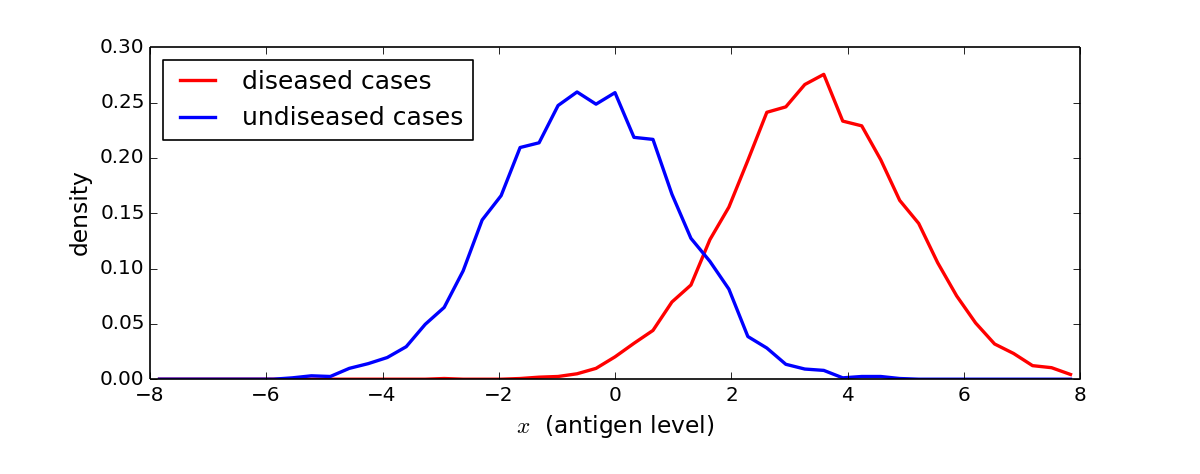
\includegraphics[width=0.9\textwidth]{disease.png}
    % Source: Original work by J. W. Miller.
  \end{center}
  \caption{Empirical distribution of $x$ for diseased and undiseased cases.}
  \label{figure:disease}
\end{figure}

The enzyme-linked immunosorbent assay (ELISA) is a chemical test for the presence of an antigen of interest. It is very widely used for the detection of diseases such as malaria, HIV, West Nile virus, and celiac disease, and can also be used to detect food allergens such as nuts, milk, and eggs.

Suppose you are using an ELISA test to detect a disease. The test produces a single number, say $x$, measuring the amount of antigen. From many previous tests, you essentially know the distribution of $x$ in each case, that is, you know $p(x|D)$ in the diseased cases (D) and $p(x|U)$ in the undiseased cases (U). See Figure \ref{figure:disease}.

You need to diagnose each future case as diseased or undiseased, based on the observed $x$. How would you make this diagnosis?


\vspace{1em}
(Think for 1 minute about roughly how you might approach this.)


\vspace{4em}
The normal (a.k.a. Gaussian) distribution $\N(\mu,\sigma^2)$ with mean $\mu$ and variance $\sigma^2$ has p.d.f.
$$ \N(x\mid \mu,\sigma^2) = \frac{1}{\sqrt{2\pi\sigma^2}}\exp\Big(-\frac{1}{2\sigma^2}(x-\mu)^2\Big). $$
Assume that
\begin{align*}
p(x|D) &=\N(x\mid \mu_D,\sigma^2) \\
p(x|U) &=\N(x\mid \mu_U,\sigma^2)
\end{align*}
where $\mu_D,\mu_U$, and $\sigma$ are all known.

\vspace{1em}
(Work on this for 10 minutes.)



\newpage
\subsection*{Solution}
This is a clear case of a decision problem with two possible actions: diagnosed as diseased (D) or undiseased (U). 
A Bayesian approach is as follows. Determine the prior probability of disease $p(D)$ (and in turn, $p(U) = 1-p(D)$); this might be possible to determine based on the previous cases, but beware of biased sampling. 
Determine the loss function $\ell$:
\begin{center}
\begin{tabular}{l r|c|c|}
\multicolumn{2}{r}{} & \multicolumn{2}{c}{Diagnosis} \\
\multicolumn{2}{r}{}
 &  \multicolumn{1}{c}{D}
 & \multicolumn{1}{c}{U} \\
\cline{3-4}
\multirow{2}{*}{Truth} 
   & D & $\ell(D,D)$ & $\ell(D,U)$ \\
   \cline{3-4}
   & U & $\ell(U,D)$ & $\ell(U,U)$ \\
   \cline{3-4}
\end{tabular}
\end{center}
Using Bayes' theorem, compute the posterior probability of disease for a given individual,
$$ p(D|x) =\frac{p(x|D) p(D)}{p(x|D) p(D) + p(x|U) p(U)}. $$
Make the diagnosis ($a=D$ or $a=U$) that minimizes the posterior expected loss,
$$ \rho(a,x) = \ell(D,a) p(D|x) + \ell(U,a) p(U|x). $$ 

It turns out that this decision rule takes a nice and simple form in which we just have to compare $x$ to a ``cut-off'' value. Assume $\mu_D>\mu_U$ (the mean antigen level for diseased is higher than undiseased), $\ell(D,U)>\ell(D,D)$ (the loss for misdiagnosing diseased cases is higher than correctly diagnosing them), and $\ell(U,D)>\ell(U,U)$ (the loss for misdiagnosing undiseased cases is higher than correctly diagnosing them).  It can be shown (with a couple pages of calculations) that the Bayes procedure is to diagnose as ``diseased'' whenever 
$$ x > c $$
and ``undiseased'' otherwise, where
$$c = \frac{\sigma^2}{\mu_D-\mu_U}\left(\frac{\mu_D^2-\mu_U^2}{2\sigma^2} +\log\frac{p(U)}{p(D)}
+\log\frac{\ell(U,D)-\ell(U,U)}{\ell(D,U)-\ell(D,D)}\right). $$

Note: If the variances of $p(x|D)$ and $p(x|U)$ are not equal, then the Bayes procedure is a little more complicated.




\newpage
\section*{Exercise 2: The speed of light}

In 1882, Simon Newcomb made 66 measurements of the amount of time it took for light to travel from his laboratory on the Potomac River, to a mirror placed at the base of the Washington Monument, and back. Converted to speed, in units of $\times 10^8$ meters/second, his data was as follows:

\begin{center}
\begin{tabular}{llllll}
2.9974 & 2.9976 & 2.9968 & 2.9979 & 2.9966 & 3.0061 \\ 
2.9975 & 2.9988 & 2.9959 & 3.0010 & 2.9973 & 2.9981 \\
2.9979 & 2.9982 & 2.9977 & 2.9971 & 2.9980 & 2.9973 \\
2.9970 & 2.9985 & 2.9979 & 2.9983 & 2.9964 & 2.9969 \\
2.9964 & 2.9974 & 2.9977 & 2.9982 & 2.9974 & 2.9973 \\
2.9963 & 2.9977 & 2.9974 & 2.9976 & 2.9971 & 2.9969 \\
2.9964 & 2.9976 & 2.9971 & 2.9981 & 2.9964 & 2.9980 \\
2.9975 & 2.9975 & 2.9974 & 2.9975 & 2.9970 & 2.9975 \\
2.9976 & 2.9968 & 2.9976 & 2.9969 & 2.9969 & 2.9979 \\
2.9960 & 2.9974 & 2.9979 & 2.9977 & 2.9969 & 2.9977 \\
2.9973 & 2.9975 & 2.9974 & 2.9973 & 2.9988 & 2.9980 \\
\end{tabular}
\end{center}
% 24.828 & 24.826 & 24.833 & 24.824 & 24.834 & 24.756 \\
% 24.827 & 24.816 & 24.84 & 24.798 & 24.829 & 24.822 \\
% 24.824 & 24.821 & 24.825 & 24.83 & 24.823 & 24.829 \\
% 24.831 & 24.819 & 24.824 & 24.82 & 24.836 & 24.832 \\
% 24.836 & 24.828 & 24.825 & 24.821 & 24.828 & 24.829 \\
% 24.837 & 24.825 & 24.828 & 24.826 & 24.83 & 24.832 \\
% 24.836 & 24.826 & 24.83 & 24.822 & 24.836 & 24.823 \\
% 24.827 & 24.827 & 24.828 & 24.827 & 24.831 & 24.827 \\
% 24.826 & 24.833 & 24.826 & 24.832 & 24.832 & 24.824 \\
% 24.839 & 24.828 & 24.824 & 24.825 & 24.832 & 24.825 \\
% 24.829 & 24.827 & 24.828 & 24.829 & 24.816 & 24.823 \\

If, like Newcomb, you were interested in determining the speed of light, how would you analyze this data?

\vspace{1em}
(Think for 1 minute about roughly how you might approach this.)


\vspace{4em}
The normal (a.k.a. Gaussian) distribution $\N(\theta,\lambda^{-1})$ with mean $\theta$ and precision (inverse variance) $\lambda = 1/\sigma^2$ has p.d.f.
$$ \sqrt{\frac{\lambda}{2\pi}}\exp\Big(-\frac{\lambda}{2}(x-\theta)^2\Big). $$
Let $\theta$ be the speed of light, and consider a normal model for Newcomb's data:
$$X_1,\dotsc,X_n\iid\N(\theta,\lambda^{-1}).$$
For simplicity, assume the precision $\lambda$ is known from extensive calibration testing.
Consider the ``improper'' uniform prior: for all $\theta$,
$$p(\theta) = 1.$$
Using Bayes' theorem in the usual way, what is the resulting posterior distribution $p(\theta|x_{1:n})$?  Give your answer in terms of $x_1,\dotsc,x_n$ (in other words, you don't need to plug in the actual values above).

\vspace{1em}
(Work on this for 10 minutes.)


\newpage
\subsection*{Solution}
One way of analyzing this data is to use a normal model, as described above. To derive the posterior, first note that 
\begin{align*}
p(x_i|\theta) & =\sqrt{\frac{\lambda}{2\pi}}\exp\Big(-\frac{\lambda}{2}(x_i-\theta)^2\Big)\\
& \propto \exp\Big(-\frac{\lambda}{2}(-2 x_i\theta + \theta^2)\Big)\\
& \propto \exp\big(\lambda x_i \theta - \tfrac{1}{2}\lambda\theta^2\big).
\end{align*}
Since we are using the flat prior $p(\theta) = 1$, the posterior is
\begin{align}
p(\theta|x_{1:n}) &\propto p(x_{1:n}|\theta)p(\theta) \notag\\
& = \prod_{i = 1}^n p(x_i|\theta)\notag\\
& \propto \exp\big(\lambda\theta\textstyle\sum x_i - \tfrac{1}{2}n\lambda\theta^2\big).\label{equation:normal}
\end{align}
Since the exponent is quadratic in $\theta$, this is proportional to a normal distribution. To find the parameters, consider a generic normal distribution on $\theta$: %, with mean $\mu$ and precision $L$:
\begin{align*}
\N(\theta|\mu,L^{-1}) &= \sqrt{\frac{L}{2\pi}} \exp\Big(-\frac{L}{2}(\theta - \mu)^2\Big) \\
&\propto \exp\big(-\tfrac{1}{2}L\theta^2 + L\theta\mu\big).
\end{align*}
This will be equal to Equation \ref{equation:normal} if
\begin{align*}
L &= n\lambda \qquad\text{ and }\\
L\mu &= \lambda\textstyle\sum x_i.
\end{align*}
Solving for $\mu$ and $L$ gives us
\begin{align*}
\mu & = \bar x= \frac{1}{n}\sum_{i=1}^n x_i \\
L &= n\lambda.
\end{align*}
Therefore,
$$ p(\theta|x_{1:n}) = \N(\theta\mid \bar x, (n\lambda)^{-1}).$$



\begin{figure}
  \begin{center}
    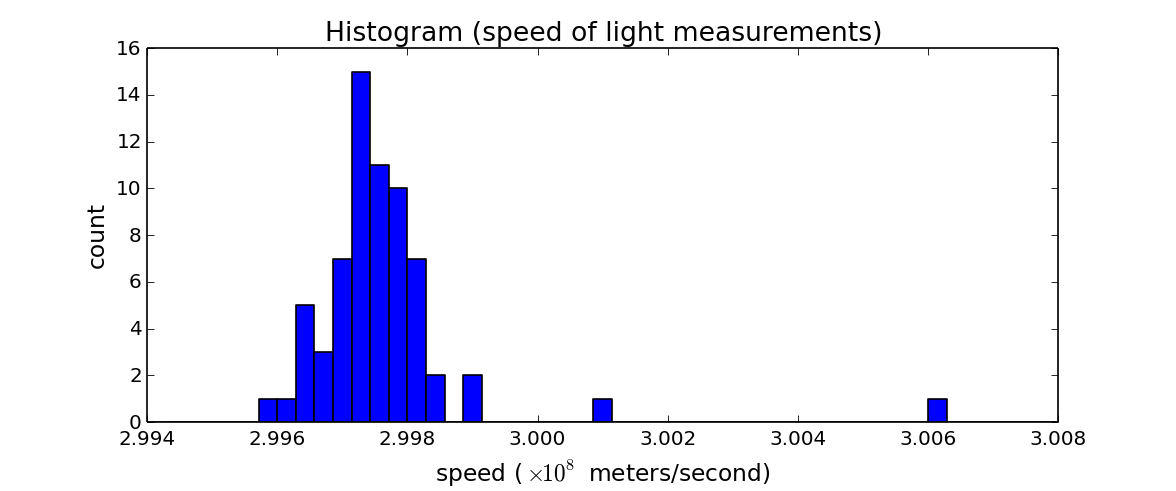
\includegraphics[width=0.9\textwidth]{newcomb-histogram.png}
    % Source: Original work by J. W. Miller.
  \end{center}
  %\caption{}
\end{figure}

\begin{figure}
  \begin{center}
    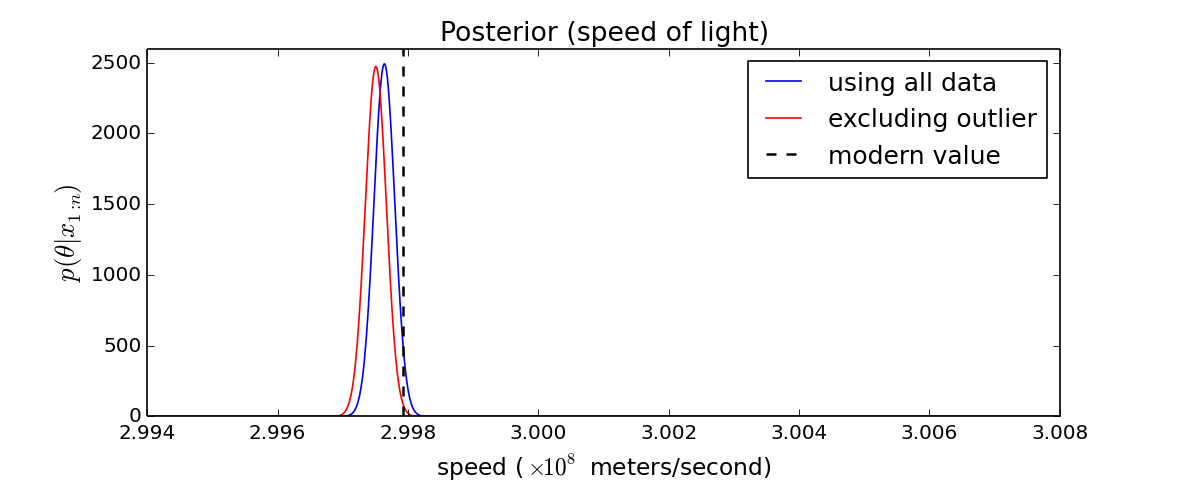
\includegraphics[width=0.9\textwidth]{newcomb-posterior.png}
    % Source: Original work by J. W. Miller.
  \end{center}
  %\caption{}
\end{figure}

\begin{figure}
  \begin{center}
    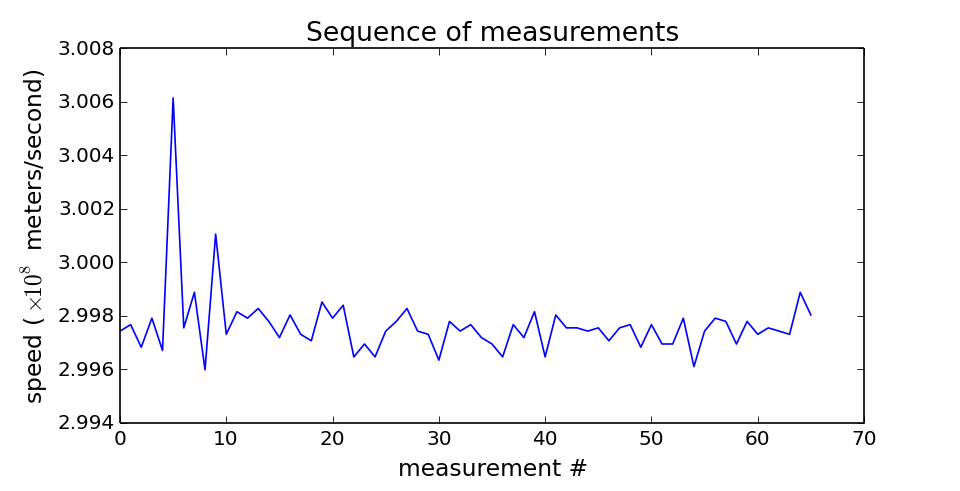
\includegraphics[width=0.8\textwidth]{newcomb-sequence.png}
    % Source: Original work by J. W. Miller.
  \end{center}
  %\caption{}
\end{figure}


\subsubsection*{Outliers}
This dataset has an outlier (or maybe two outliers) relatively far away from the majority of the observations. This is difficult to see from the data alone, but apparent from the histogram. It's always important to visualize your data---it is said that the statistician's best tool is the eye.

If the extreme outlier (3.0061) is removed, then the posterior is noticeably shifted to the left.  This illustrates that a normal model is sensitive to outliers. In fact, even one outlier---if sufficiently far away---can have an arbitrarily large effect on the posterior. To deal with this, sometimes people use a generating distribution with ``heavier tails'', such as Student's t-distribution or the Laplace (a.k.a. double exponential) distribution, instead of the normal distribution. However, these are not as easy to use, computationally.

\subsubsection*{Improper priors}
An \term{improper prior} is a nonnegative function $p(\theta)$ which is not a p.d.f.\ because it does not have a finite integral, in other words, $\int p(\theta) d\theta = \infty$. The choice of $p(\theta) = 1$, for $\theta\in\R$, is an example of an improper prior.

Even though an improper prior is not actually a prior at all (since it does not correspond to a probability distribution), we can still try to plug it into Bayes' theorem as though it were---in other words, we can define the posterior to be proportional to $p(x|\theta) p(\theta)$. It turns out that in many cases (but not always) this is normalizable, and thus, results in a ``proper'' posterior.



% \subsubsection*{Systematic errors / batch effects}

% Newcomb's measurements were impressively accurate, but they do seem to have a slight bias compared to the modern accepted value.  How could this be?  Perhaps he slightly mismeasured the distance.  Perhaps his equipment had some undetected bias.  There are many things that could go slightly wrong.  As more and more measurements are taken, the posterior inexorably concentrates---but if there are systematic errors, typically it will not concentrate at the correct place.  This is particularly noticeable when comparing results from different experimenters or different laboratories. For instance, Figure \ref{figure:batch} shows several different estimates of the speed of light, along with confidence intervals (figure due to Rafael Irizarry).

%The current accepted value is 670,616,629 mph.
%299,792,458 meters/second.


% \begin{figure}
  % \begin{center}
    % 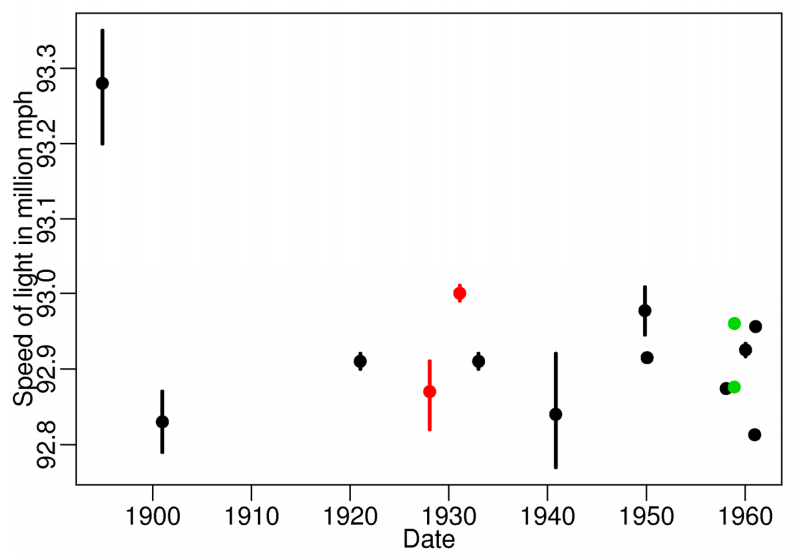
\includegraphics[width=0.5\textwidth]{batch2.png}
    %% Source: Youden, W. J. (1972). Enduring values. Technometrics, 14(1), 1-11.
    %% License: ???
  % \end{center}
  % \caption{Measurements of the speed of light with the reported errors. (Youden, 1972)}
  % \label{figure:batch}
% \end{figure}















\section*{References and supplements}

% \subsubsection*{}
\begin{itemize}
%\item Jahn, R.G., B.J. Dunne and R.D. Nelson. 1987. \textit{Engineering anomalies research}. Journal of Scientific Exploration 1:21�50.
\item Youden, W. J. (1972). Enduring values. Technometrics, 14(1), 1-11.
\end{itemize}



\end{document}









\newpage
\section*{Exercise 3: Extrasensory perception (ESP) experiment}

Jahn, Dunne and Nelson (1987) tested a man who claimed to be able to control the output of a random number generator using only his mind (``psychokinesis''). The random number generator was supposed to output 0 or 1 with equal probability, unless the man could control it, in which case it would be biased.  

In the test, 104,490,000 numbers were generated, and 52,263,471 of these were ones (the rest were zeros).  How would you assess whether or not this provides evidence for psychokinesis?

\vspace{1em}
(Work on this for 10 minutes.)

\newpage
\subsection*{Solution}
This is a surprisingly subtle example. There is more than one way to approach the problem, and different ways give different answers. For all of the approaches, we model the number of ones as $X\sim\Binomial(n,\theta)$, where $n =$ 104,490,000, and we observe $x =$ 52,263,471. (Note that it would be equivalent to model the sequence as $X_1,\dotsc,X_n\sim\Bernoulli(\theta)$.) First, we describe two frequentist approaches, as a point of reference.

\subsubsection*{Frequentist approach 1: Hypothesis test}
From the classical frequentist perspective, this is a hypothesis test:
\begin{itemize}
\item[] $H_0: \theta = \theta_0$ (no psychokinesis)
\item[] $H_1: \theta\neq \theta_0$ (psychokinesis)
\end{itemize}
where $\theta_0 = 0.5$. The standard approach is to consider the test statistic
$$ T(X) = \frac{X/n - \theta_0}{\sigma(X/n)} $$
where $\sigma(\cdot)$ denotes standard deviation, 
and use a normal approximation to approximate the p-value:
$$p = \Pr\big(|T(X)|\geq |T(x)|\mid \theta_0\big).$$
This gives us $p \approx 0.0003$, which is in the range usually considered significant. This would seem to provide evidence for the man's claim of psychokinesis.

\subsubsection*{Frequentist approach 2: Estimate the effect size}
Even though the result is statistically significant, it might not be considered ``practically significant''. To assess this, we can consider the size of the effect by computing a 95\% confidence interval:
$$x/n \pm 1.96\sigma(X/n)$$
as shown in Figure \ref{figure:ESP}. This is so close to 0.5 that we might not consider it to be practically significant.

\begin{figure}
  \begin{center}
    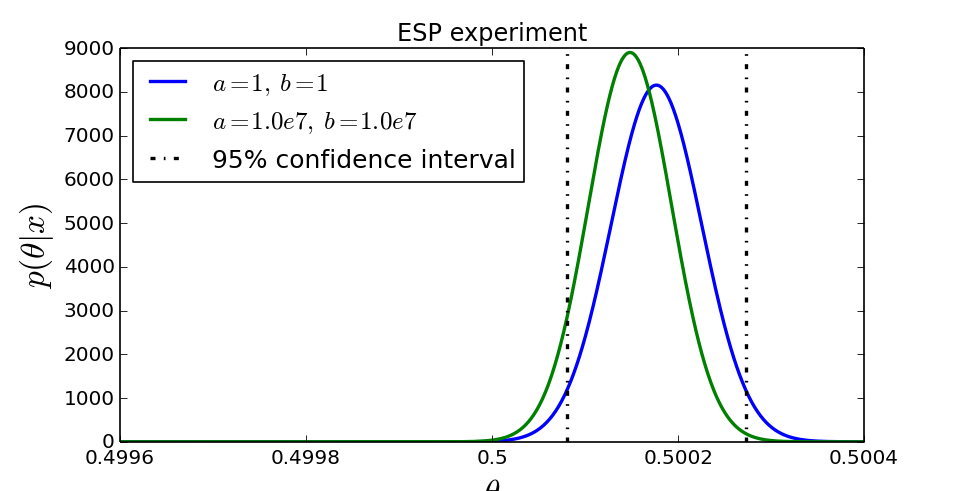
\includegraphics[width=0.85\textwidth]{ESP.png}
    % Source: Original work by J. W. Miller.
  \end{center}
  \caption{}
  \label{figure:ESP}
\end{figure}


\subsubsection*{Sort-of-Bayesian approach}
A more Bayesian approach would be to put a prior on $\theta$, and consider the posterior. For example, suppose we take a $\Beta(a,b)$ prior. Then the posterior is $\Beta(a + x, b + n-x)$; see Figure \ref{figure:ESP} for the posterior with a relatively non-informative choice of $a,b$ ($a = 1$, $b = 1$). We can compute a Bayesian confidence interval (a.k.a. a credible interval) by choosing an interval $[u,v]$ such that
$$\Pr(u\leq \theta\leq v\mid X=x) = 0.95. $$
In this example, the frequentist 95\% confidence interval has this property (almost exactly).

In order to demonstrate just how insensitive the posterior is to the prior, Figure \ref{figure:ESP} also shows the posterior for a very informative choice of $a,b$ ($a = 10^7$, $b = 10^7$). Choices of $a,b$ less than 1 yield a posterior that is indistinguishable from choosing $a = 1$, $b = 1$.


\subsubsection*{Fully Bayesian approach}
The fully Bayesian approach is to put a prior on the hypotheses:
\begin{itemize}
\item[] $H_0: \theta = \theta_0$ (no psychokinesis)
\item[] $H_1: \theta\neq \theta_0$ (psychokinesis)
\end{itemize}
where $\theta_0 = 0.5$, and in the case of $H_1$, put a prior on $\theta$. For instance, suppose we consider the two hypotheses equally likely \textit{a priori},
$$ p(H_0) = p(H_1) = 1/2$$
and put a Beta prior on $\theta$ in the case of $H_1$,
$$\theta|H_1\,\sim\Beta(a,b).$$
By Bayes' theorem,
\begin{align}\label{equation:Bayes}
p(H_0|x) =\frac{p(x|H_0) p(H_0)}{p(x|H_0) p(H_0)+p(x|H_1) p(H_1)}.
\end{align}
In the case of $H_0$ (no psychokinesis),
\begin{align*}
p(x|H_0) = {n\choose x} \theta_0^x(1-\theta_0)^{n-x} = {n\choose x}(1/2)^n.
\end{align*}
In the case of $H_1$ (psychokinesis), we need to integrate $\theta$ out in order to compute $p(x|H_1)$. In other words, we need to compute the marginal likelihood:
\begin{align*}
p(x|H_1) & =\int p(x|\theta,H_1) p(\theta|H_1) d\theta\\
& = {n\choose x}\frac{B(a + x,b + n-x)}{B(a,b)}.
\end{align*}
Plugging these into Equation \ref{equation:Bayes}, we get the posterior probability of each hypothesis. Here are the results for different values of $a,b$:
\begin{align*}
a=b=10^0 \qquad & p(H_0|x) = 0.92 \\
a=b=10^1 \qquad & p(H_0|x) = 0.77 \\
a=b=10^2 \qquad & p(H_0|x) = 0.51 \\
a=b=10^3 \qquad & p(H_0|x) = 0.25 \\
a=b=10^4 \qquad & p(H_0|x) = 0.10
\end{align*}
For certain choices---e.g., $a = 1$ and $b = 1$---the posterior supports $H_0$ (no psychokinesis), while for bigger $a,b$, it supports $H_1$ (psychokinesis).  Note that the hypotheses have equal prior probability in each of these cases---thus, the prior on $\theta$ has a strong influence on the result!

The reason why this happens is that when $a=b$ and they are relatively large, the prior is more concentrated around 0.5, and since $x/n$ is so near 0.5, the data appear to be more plausible under hypothesis $H_1:\theta\neq \theta_0$. Will this trend continue as $a$ and $b$ increase? What do you think? Why?


\subsubsection*{Barlett--Lindley paradox}
This example illustrates the Barlett--Lindley paradox: entirely reasonable frequentist and Bayesian procedures can give entirely different answers. Basically, it boils down to this: when doing Bayesian hypothesis testing, the prior on parameters really matters. This also comes up in model selection problems.


\subsubsection*{Other explanations}
Can you think of other reasons that could explain this data?  One possibility is that the random number generator was actually biased.  To address this, a control experiment could be run without the man trying to influence the outcome.  It could also be a case of p-hacking, for instance, collecting more and more data until a small p-value was obtained.




%\newpage
%\section{Comparing birthrates}


